\section{Introduction}
\label{sec:introduction}

Graphics processing units (GPUs) are becoming powerful many-core compute
devices.
For example, NVIDIA GPUs integrate more than $1,500$ processing cores on
a single chip and the peak double-precision performance exceeds 1
TFLOPS while sustaining thermal design power (TDP) in the same order of
magnitude as traditional multicore CPUs~\cite{NVIDIA_Kepler}. 
This rapid growth of GPUs is due to recent advances in the
programming model, often referred to as general-purpose computing on
GPUs (GPGPU).
Data-parallel and compute-intensive applications receive signficant
performance benefits using GPGPU.
Currently a main application of GPGPU is supercomputing~\cite{TOP500}
but there are more and more emerging applications in different fields.
Examples include plasma control~\cite{Kato_ICCPS13}, autonomous
driving~\cite{McNaughton_ICRA11}, software routing~\cite{Han_SIGCOMM10},
encrypted networking~\cite{Jang_NSDI11}, and storage
management~\cite{Bhatotia_FAST12, Gharaibeh_HPDC10, Kato_ATC12,
Sun_SYSTOR12}.
This broad range of applications raises the need of further developing
GPU technology to support scalablability of emerging data-parallel and
compute-intensive applications.

\begin{figure}[!t]
 \centering
 \subfigure[Host to Device]{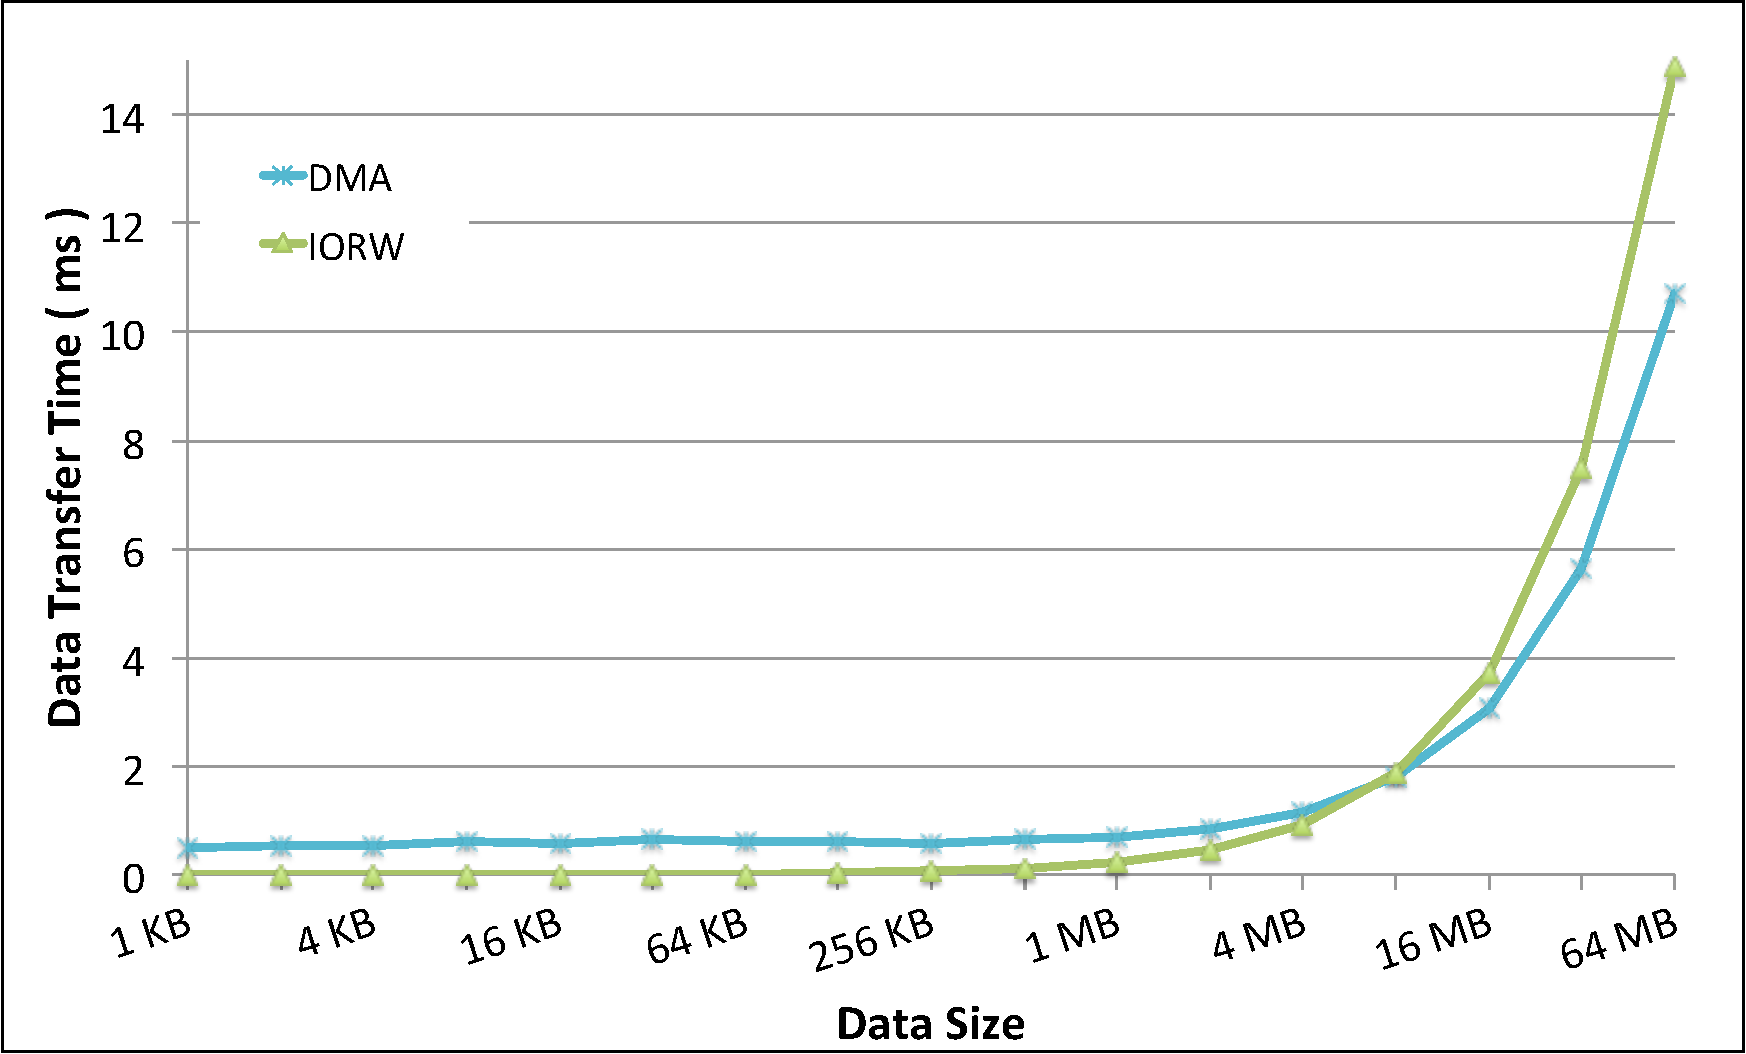
\includegraphics[width=0.34\textwidth]{figure/Graph/forIntro_HtoD.pdf}}\\
 \subfigure[Device to Host]{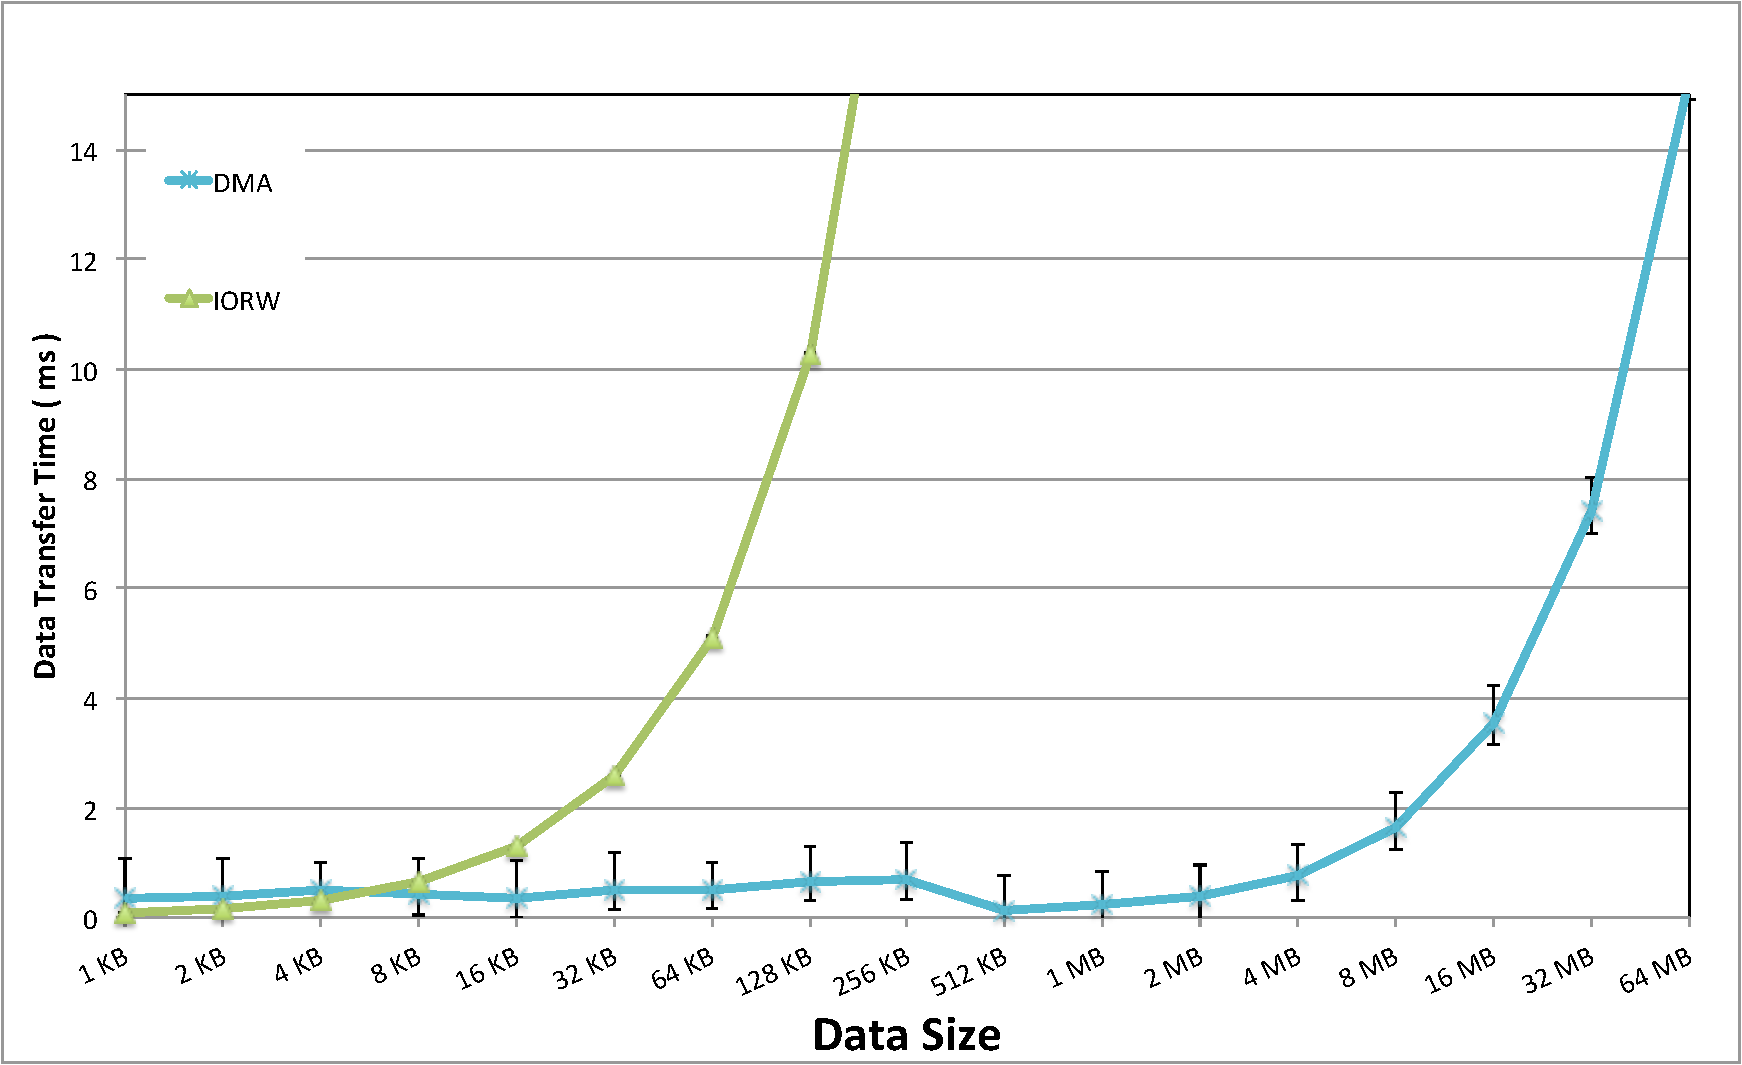
\includegraphics[width=0.34\textwidth]{figure/Graph/forIntro_DtoH.pdf}}
 \caption{Performance of DMA and I/O read/write for the GPU.}
 \label{fig:intro_data_transfer}
\end{figure}

One of the greatest challenges of GPU computing is the integration of
predictable real-time systems.
So far the real-time systems community has addressed resource management
issues of GPUs~\cite{Basaran_ECRTS12, Elliott_RTS12, Elliott_ECRTS12,
Kato_ATC11, Kato_RTAS11, Kato_RTSS11}.
The main contribution of these work is the scheduling of compute
kernels and data transfers associated with the GPU.
On the other hand, the basic performance and latency issues of these
operations are not explored in the real-time systems literature.
Given that compute kernels are offloaded to the GPU, their performance
and latency are more dominated by compiler and hardware technology.
However, optimization of data transfers must be complemented by system
software due to constrants of PCIe devices~\cite{Kato_ATC12}.

performance of compute kernels is not a scope of resource management
issues, but that of data transfers is managable~\cite{Kato_ATC12}.

GPU computing in the current state of the art involves many black-box
pieces.
Open-source projects have revealed key mechanisms of GPU
resource management~\cite{Kato_ATC11, Kato_ATC12}, but the hardware
details of GPUs are not disclosed to the public.
Current systems hence rely on a high-level programming framework and
limited information of proprietary sofware provided by the GPU
vendors.
This black box constraint may be acceptable for throughput-oriented
high-performane computing but 
One of the mysteries of GPU computing due to this black box constraint
is \textit{how to transfer data between the host and the device memory}.
In typical GPU-accelerated systems, the CPU executes a master flow of
the program using the host memory while the GPU executes a compute
kernel using the device memory.
This heterogeneity of GPU computing requires the program to exchange
data between the host and the device memory.
A programming framework often provides a set of data transfer methods as
part of an application programming interface (API), but their mechanisms
are encapsulated in the proprietary software implementation.

We must pray that these data transfer methods are already optimized by
the vendors.

One of the greatest challenges of GPU computing is the management of
latency issues.

nobody knows